\documentclass{beamer}

%%%%%%%%%%%%%%%%%%%%%%%%%%%%%%%%%%%%%%%%%%%%%%%%%%%%%%%%%%%%%%%%%%%%%%%%%%%%%%%%
% DEFINITIONS AND PACKAGES
%%%%%%%%%%%%%%%%%%%%%%%%%%%%%%%%%%%%%%%%%%%%%%%%%%%%%%%%%%%%%%%%%%%%%%%%%%%%%%%%

% Languages.
\usepackage[utf8]{inputenc}
\usepackage[english]{babel}
\usepackage[numberedbib]{apacite}
\usepackage{tikz}
\selectlanguage{english}

% Miscellaneous.
\usepackage{hyperref}
\usepackage{array,multirow}

% Path to the figures directory.
\graphicspath{{figures/}}

%%%%%%%%%%%%%%%%%%%%%%%%%%%%%%%%%%%%%%%%%%%%%%%%%%%%%%%%%%%%%%%%%%%%%%%%%%%%%%%%
% TITLE SLIDE
%%%%%%%%%%%%%%%%%%%%%%%%%%%%%%%%%%%%%%%%%%%%%%%%%%%%%%%%%%%%%%%%%%%%%%%%%%%%%%%%

\title[A Computational Platform for Gene Expression Analysis]{A Computational Platform\\for Gene Expression Analysis}
\author[Diogo Teixeira]{
  Diogo Teixeira\\[1ex]
  {\footnotesize Supervisors: Rui Camacho\inst{1}, Nuno Fonseca\inst{2}}
}
\institute[FEUP]
{
  \inst{1}
  LIAAD INESC, Porto \& DEI FEUP, Universidade do Porto, Porto
  \and
  \inst{2}
  EMBL-EBI, Cambridge, UK
}
\date{July 2014}
\subject{Informatics, Biology}

%%%%%%%%%%%%%%%%%%%%%%%%%%%%%%%%%%%%%%%%%%%%%%%%%%%%%%%%%%%%%%%%%%%%%%%%%%%%%%%%
% STYLE
%%%%%%%%%%%%%%%%%%%%%%%%%%%%%%%%%%%%%%%%%%%%%%%%%%%%%%%%%%%%%%%%%%%%%%%%%%%%%%%%

\makeatletter
\usetheme{Luebeck}
\usecolortheme{beaver}
\usefonttheme{serif}
\setbeamerfont{footline}{size=\fontsize{4}{12}\selectfont}
\setbeamertemplate{navigation symbols}{}
\setbeamertemplate{headline}{}
\setbeamertemplate{footline}
{%
  \leavevmode%
  \hbox{\begin{beamercolorbox}[wd=.23\paperwidth,ht=3.0ex,dp=2.0ex,center]{author in head/foot}%
      \usebeamerfont{author in head/foot}\insertshortauthor%
    \end{beamercolorbox}%
    \begin{beamercolorbox}[wd=.65\paperwidth,ht=3.0ex,dp=2.0ex,center]{title in head/foot}%
      \usebeamerfont{title in head/foot}\insertshorttitle
    \end{beamercolorbox}%
    \begin{beamercolorbox}[wd=.12\paperwidth,ht=3.0ex,dp=2.0ex,center]{author in head/foot}%
      \usebeamerfont{author in head/foot} \insertframenumber{} / \inserttotalframenumber
    \end{beamercolorbox}}%
  \vskip0pt
}

%%%%%%%%%%%%%%%%%%%%%%%%%%%%%%%%%%%%%%%%%%%%%%%%%%%%%%%%%%%%%%%%%%%%%%%%%%%%%%%%
% DOCUMENT
%%%%%%%%%%%%%%%%%%%%%%%%%%%%%%%%%%%%%%%%%%%%%%%%%%%%%%%%%%%%%%%%%%%%%%%%%%%%%%%%

\begin{document}

% Title slide.
\frame{\titlepage}

% TOC.
\begin{frame}
  \frametitle{Outline}
  \tableofcontents
\end{frame}

%%%%%%%%%%%%%%%%%%%%%%%%%%%%%%%%%%%%%%%%%%%%%%%%%%%%%%%%%%%%%%%%%%%%%%%%%%%%%%%%
% INTRODUCTION
%%%%%%%%%%%%%%%%%%%%%%%%%%%%%%%%%%%%%%%%%%%%%%%%%%%%%%%%%%%%%%%%%%%%%%%%%%%%%%%%

\section{Introduction}
\subsection{Domain Problem}
\begin{frame}[allowframebreaks]
  \frametitle{Domain Problem}
  \framesubtitle{Introduction}

\begin{itemize}
\item
Molecular biology is a young field of study, with a lot of unknowns and partial
knowledge.\\ \vspace{0.8cm}

\item
Studying gene expression is crucial to understand the mechanisms that control
living organisms.\\ \vspace{0.8cm}

\item
We focused on two different areas:
\begin{itemize}
  \item
  differential expression analysis;

  \item
  RNA-binding protein (RBP) discovery and analysis.
\end{itemize}
\end{itemize}

\framebreak

Three distinct problems:\\ \vspace{0.5cm}

\begin{itemize}
\item
Read alignment against a reference genome and differential expression analysis
on the aligned data.\\ \vspace{0.7cm}

\item
RBP discovery, analysis and information enrichment.\\ \vspace{0.7cm}

\item
Further result analysis using data mining techniques.

\end{itemize}

%NOTES:\\
%- Molecular biology is a new subject.\\
%- Many unknowns.\\
%- Gene expression is important...\\
%- Two areas of interest of IBMC experts: differential expression and RBPs.\\

\end{frame}

\subsection{Motivation and Objectives}
\begin{frame}
  \frametitle{Motivation and Objectives}
  \framesubtitle{Introduction}

\begin{columns}[<options>]
  \begin{column}{0.45\textwidth}
    \textcolor<5-6>{gray!40}{\textcolor<2-3>{gray!40}{\textbf{Tools are complex}\scriptsize\\
    Tools for biological data analysis often require a very technical set of
    skills.\\
    \vspace{0.8cm}}}

    \textcolor<6>{gray!40}{\uncover<2->{\textcolor<3-4>{gray!40}{\textbf{Tasks are repetitive}\scriptsize\\
    Analysing high quantities of data can be repetitive, especially if executed
    manually.\\
    \vspace{0.8cm}}}}

    \uncover<3->{\textcolor<4-5>{gray!40}{\textbf{Information is scattered}\scriptsize\\
    Information is easy to acquire, but is often scattered through multiple
    platforms, services and institutions.\\
    }}
  \end{column}

  \begin{column}{0.45\textwidth}
    \uncover<4-6>{\textcolor<5->{gray!40}{\textbf{Create simpler tools}\scriptsize\\
    Any user should be able to use the tools, with little to no training.\\
    \vspace{1.1cm}}}

    \uncover<5-6>{\textcolor<6->{gray!40}{\textbf{Automate tasks}\scriptsize\\
    Automated systems should perform repetitive tasks, so that users can
    focus on their work.\\
    \vspace{0.8cm}}}

    \uncover<6>{\textbf{Gather information}\scriptsize\\
    Information should be contextually aggregated, allowing for quick access of
    relevant information.
    }
  \end{column}
\end{columns}

%NOTES:\\
%Motivation:\\
%- Many tools require a very technical set of skills (tools should be facilitators, not hindrances)\\
%- Some tasks need automation.\\
%- Lots of information, often scattered in multiple places.\\
%Objectives:\\
%- Build simples tools that require minimal skill.\\
%- Automate processes.\\
%- Aggregate as much relevant information as possible.\\

\end{frame}

%%%%%%%%%%%%%%%%%%%%%%%%%%%%%%%%%%%%%%%%%%%%%%%%%%%%%%%%%%%%%%%%%%%%%%%%%%%%%%%%
% SOLUTION
%%%%%%%%%%%%%%%%%%%%%%%%%%%%%%%%%%%%%%%%%%%%%%%%%%%%%%%%%%%%%%%%%%%%%%%%%%%%%%%%

\section{Developed Solution}
\subsection{Overview}
\begin{frame}
  \frametitle{Overview}
  \framesubtitle{Developed Solution}

\begin{itemize}

\item
Two distinct problems warrant two different solutions.\\ \vspace{0.8cm}

\item
The developed system should be available anywhere, through the internet.\\ \vspace{0.8cm}

\item
The system should be as modular as possible, to allow future extensions.

\end{itemize}

%NOTES:\\
%- Two computer systems, one for each domain problem.\\
%- Both accessible through the web.\\
%- Focus on small system footprint, deployable by machine, department, institution.\\

\end{frame}

\subsection{RNA-Seq Analysis Pipeline}
\begin{frame}[allowframebreaks]
  \frametitle{RNA-Seq Analysis Pipeline}
  \framesubtitle{Developed Solution}

\begin{itemize}\small
\item
Uses iRAP as the analysis pipeline.

\item
Conducts multiple differential expression analyses with different tools.

\item
Combines results from multiple tools.
\end{itemize}

\begin{figure}
  \centering
  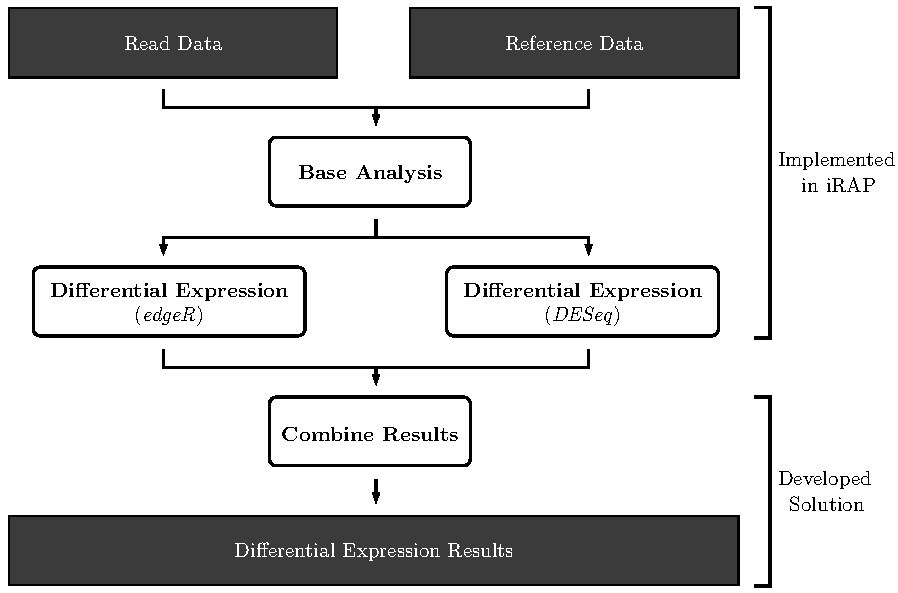
\includegraphics[width=0.65\textwidth]{tool1}
\end{figure}

%\framebreak

%Additional features:

%\begin{itemize}
%\item
%Access to iRAP's web reports and gene browser, along with result visualization
%in the web interface.\\ \vspace{0.4cm}

%\item
%Synchronization with Ensembl's reference genome repositories.\\ \vspace{0.4cm}

%\item
%Graphical job configuration.\\ \vspace{0.4cm}

%\item
%Possibility to easily include other differential expression tools.
%\end{itemize}

%NOTES:\\
%- Show scheme, refer iRAP, the script and the web interface.\\
%- Refer multiple differential expression tools.\\
%- Refer user input and tool configuration.\\

\end{frame}

\subsection{RBP Analysis Pipeline (PBS Finder)}
\begin{frame}[allowframebreaks]
  \frametitle{RBP Analysis Pipeline (PBS Finder)}
  \framesubtitle{Developed Solution}

\begin{itemize}
\item
Uses Ensembl and NCBI to identify gene species, obtain basic information and
extract genetic sequences (5' UTR, 3' UTR, 3' UTR downstream).
\end{itemize}\vspace{0.23cm}

\begin{figure}
  \centering
  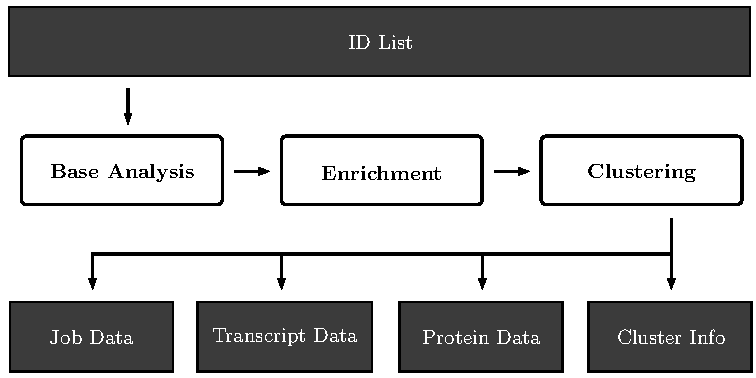
\includegraphics[width=0.65\textwidth]{workflow2}
\end{figure}

\framebreak

\begin{itemize}
\item
Uses RBPDB to discovery RNA binding proteins based on the obtained sequences.

\item
Uses UniProt to enrich the obtained results and performs clustering analysis on
those results.
\end{itemize}

\begin{figure}
  \centering
  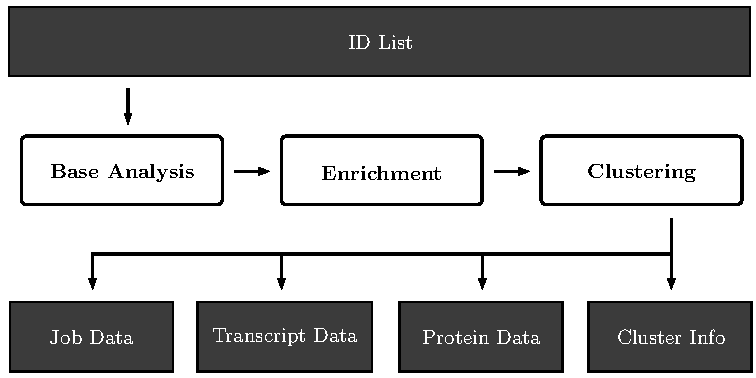
\includegraphics[width=0.65\textwidth]{workflow2}
\end{figure}

\framebreak

Clustering analysis:
\begin{itemize}
\item
Uses $k$-medoids and hierarchical clustering, both with Jaccard and binary
distance matrices.

\item
Executes every possible combination of clustering setups (alternates algorithms,
distance matrices, used features, etc.).

\item
Results are filtered (acceptable solutions must have a minimum percentage of
entries per cluster, clusters must have defining features, etc.).

\item
Solution quality internally determined based on the average silhouette.
\end{itemize}

%\framebreak

%Additional features:
%\begin{itemize}
%\item
%User account and job management system.\\ \vspace{0.3cm}

%\item
%References to external platforms with relevant information based on context.\\ \vspace{0.3cm}

%\item
%Support for multiple identifier notations (Ensembl, Entrez, RefSeq and GenBank).\\ \vspace{0.3cm}

%\item
%Visualization of defining features for each cluster.\\ \vspace{0.3cm}

%\item
%Job completed notification system.
%\end{itemize}

%NOTES:\\
%- Show scheme, RBP finding, gene enrichment, clustering.\\
%- Refer web interface.
%- Refer that the tools is in production for several months, being extensively tested by experts.\\
%- Refer user input and tool configuration.\\

\end{frame}

\subsection{Integration}
\begin{frame}
  \frametitle{Integration}
  \framesubtitle{Developed Solution}

\only<1-2>{
While focusing on aggregation and quick access to information, does it make
sense to separate the results into two different platforms?}

\only<1>{
\begin{figure}
  \centering
  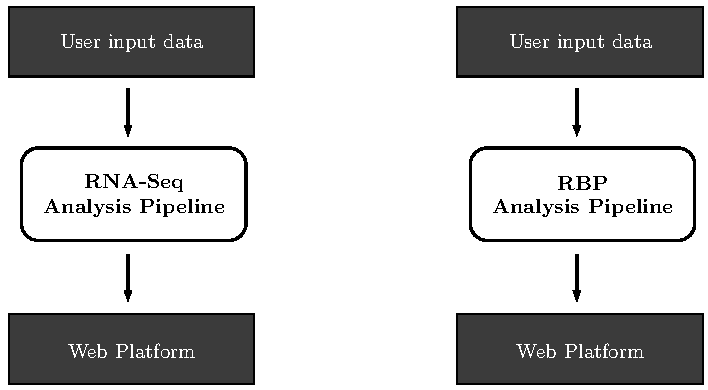
\includegraphics[width=0.8\textwidth]{integration1}
\end{figure}}

\only<3-4>{
A list of differentially expressed genes is not very useful without further
information about those genes. Does it make sense for a user to launch a new
gene enrichment task by hand?}

\only<2-3>{
\begin{figure}
  \centering
  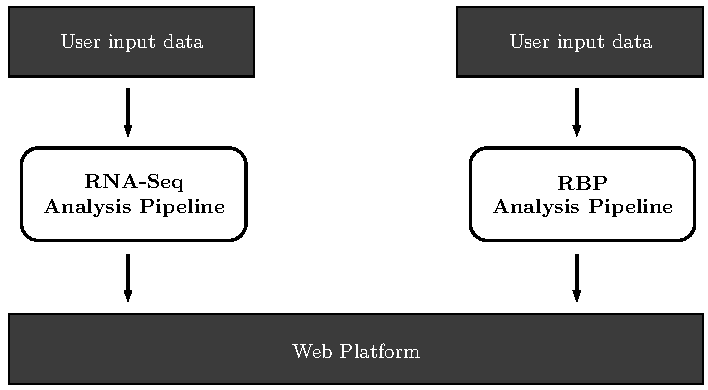
\includegraphics[width=0.8\textwidth]{integration2}
\end{figure}}

\only<5>{
A fully integrated solution: the analysis pipelines can be used separately or
automatically executed in sequence; result visualization for both pipelines is
isolated.}

\only<4-5>{
\begin{figure}
  \centering
  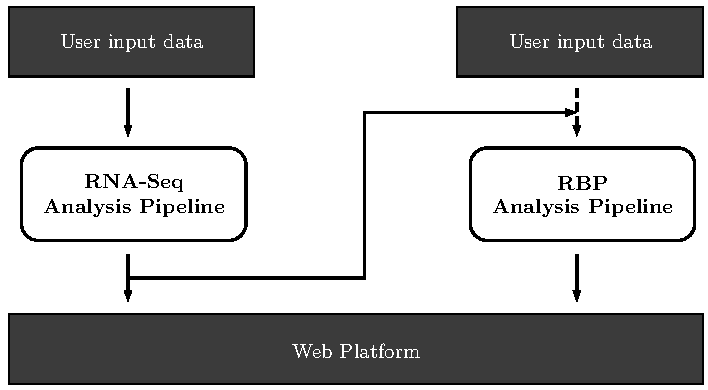
\includegraphics[width=0.8\textwidth]{integration3}
\end{figure}}

%NOTES:\\
%- Differential expression analysis could benefit from gene enrichment.\\
%- Do we really need two separate platforms?\\
%- Joined together, user choses what analysis to perform.\\
%- Still separate viewing experiences.\\

\end{frame}

%%%%%%%%%%%%%%%%%%%%%%%%%%%%%%%%%%%%%%%%%%%%%%%%%%%%%%%%%%%%%%%%%%%%%%%%%%%%%%%%
% CASE STUDIES
%%%%%%%%%%%%%%%%%%%%%%%%%%%%%%%%%%%%%%%%%%%%%%%%%%%%%%%%%%%%%%%%%%%%%%%%%%%%%%%%

\section{Case Studies}
\subsection{RNA-Seq Analysis Pipeline}
\begin{frame}[allowframebreaks]
  \frametitle{RNA-Seq Analysis Pipeline}
  \framesubtitle{Case Studies}

%NOTES:\\
%- Refer objectives, data and experimental method.\\
%- Refer results.\\

Objective
\begin{itemize}
\item
Ascertain if combining the results of multiple tools has impact on the set of
differentially expressed genes.
\end{itemize}\vspace{0.8cm}

Data set
\begin{itemize}
\item
Reproduction of ArrayExpress experiment E-GEOD-48829 (\emph{Escherichia coli}).

\item
Reference genome obtained from Ensembl Genomes and read data obtained from ENA
Sequence Read Archive.
\end{itemize}

\framebreak

Results (number of differentially expressed genes)
\begin{table}[!htb]\footnotesize
  \centering
  \begin{tabular}{{l} | {c}{c}{c}}
    & \textbf{\emph{Raw results}} & \textbf{\emph{Filtered results}} &
    \textbf{\emph{Combined results}}\\ \hline
    \textbf{\emph{edgeR}} & 4494 & 386 & \multirow{2}{*}{191}\\
    \textbf{\emph{DESeq}} & 4494 & 204 \\ \hline
  \end{tabular}
\end{table}\vspace{0.6cm}

Conclusions
\begin{itemize}
\item
Combining results impacts the final differentially expressed gene list by
reducing its size.

\item
The combined results will hopefully give researchers an higher confidence in the
experimental results.
\end{itemize}

\end{frame}

\subsection{RBP Analysis Pipeline (PBS Finder)}
\begin{frame}[allowframebreaks]
  \frametitle{RBP Analysis Pipeline (PBS Finder)}
  \framesubtitle{Case Studies}

Objectives
\begin{itemize}
\item
Assess the general usefulness of PBS Finder.

\item
Compare PBS Finder with the existing techniques of manual analysis.

\item
Assess the impact of differences in hardware performance in the overall
performance of the platform.
\end{itemize}\vspace{0.8cm}

Data set
\begin{itemize}
\item 23 genes from the \emph{RhoGTPase} family (\emph{Rattus norvegicus})
provided by IBMC.
\end{itemize}

\framebreak

Results (expert estimation of 30 minutes per gene analysed)
\begin{table}[!htb]\footnotesize
  \centering
  \begin{tabular}{{l} | {l}{l}{l}}
    \textbf{\emph{Number of IDs}} & \textbf{\emph{Machine1}} & \textbf{\emph{Machine2}} & \textbf{\emph{Manual method}} \\ \hline
    100  & $9m\ 56s$          & $11m\ 1s$      & $\approx 50h$\\
    500   & $41m\ 47s$         & $55m\ 51s$     & $\approx 250h$\\
    900   & $1h\ 33m\ 32s$     & $2h\ 7m\ 4s$   & $\approx 450h$\\ \hline
  \end{tabular}
\end{table}\vspace{0.3cm}

Conclusions
\begin{itemize}
\item
PBS Finder can reproduce the results an expert would get.

\item
Months worth of an expert's manual work can be accomplished in a few hours.

\item
While hardware performance has a significant impact on analysis time, the
platform achieves satisfactory performance on personal computer-level hardware.
\end{itemize}

\framebreak

Results (viewed in PBS Finder)\\
\begin{figure}
  \centering
  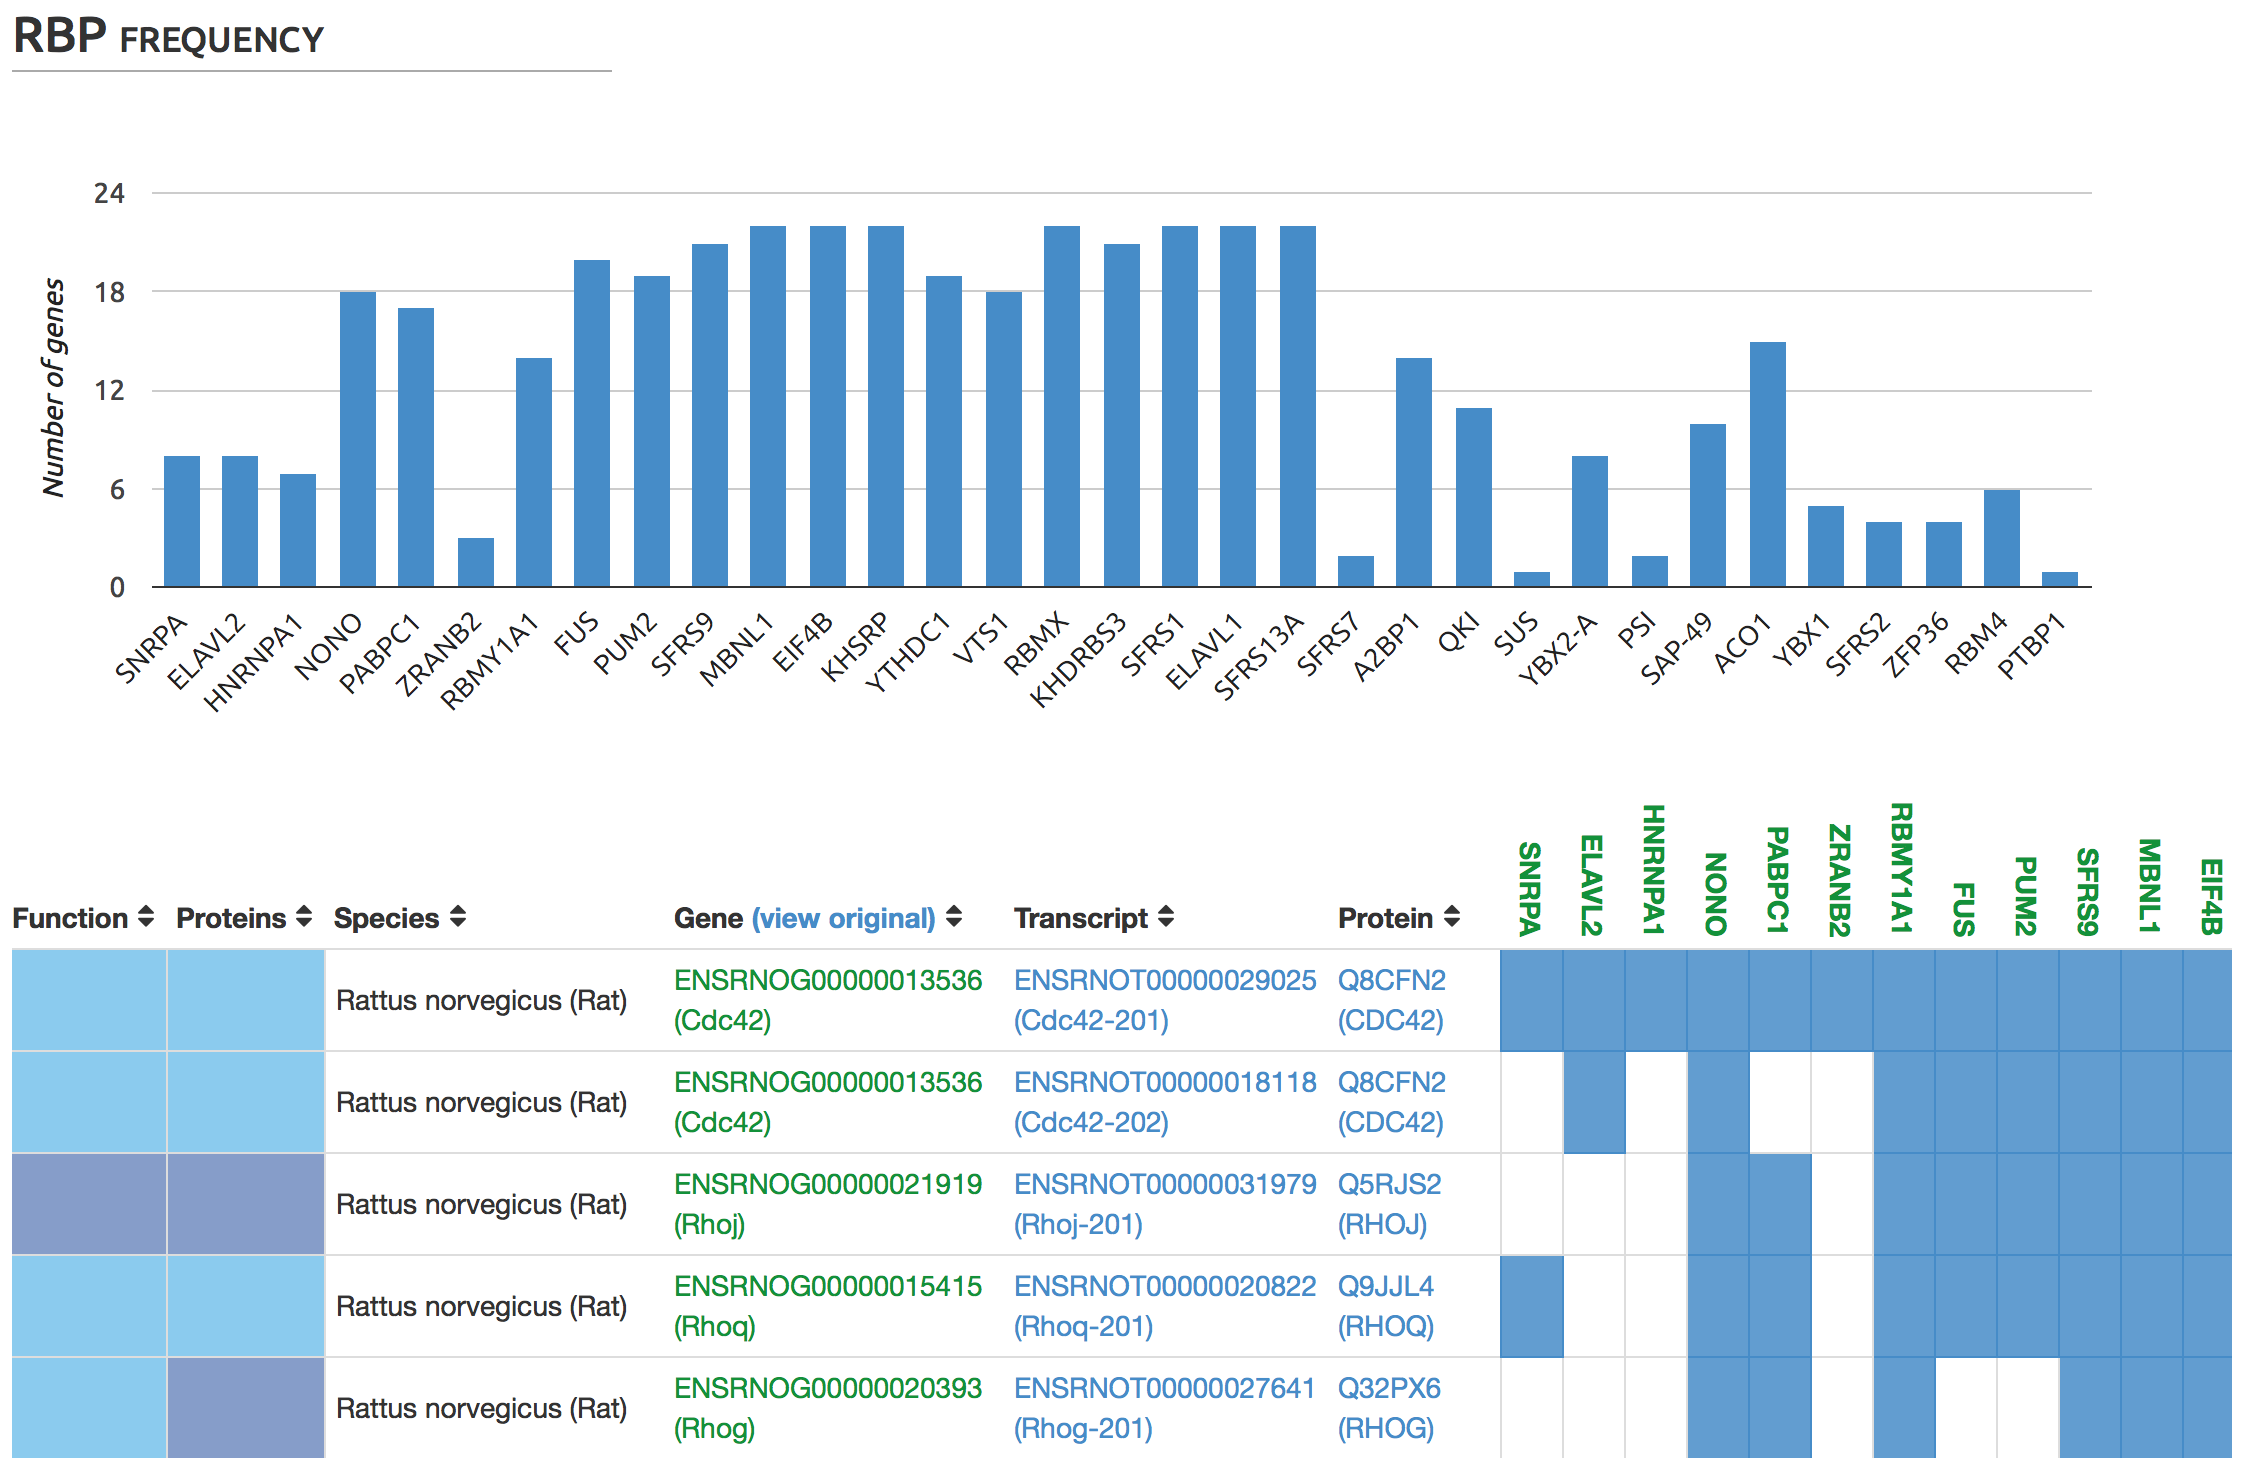
\includegraphics[width=0.85\textwidth]{job_view}
\end{figure}

%NOTES:\\
%- Refer objectives, data and experimental method.\\
%- Refer results.\\
%- Show screenshot.\\
%- Show table.\\

\end{frame}

%%%%%%%%%%%%%%%%%%%%%%%%%%%%%%%%%%%%%%%%%%%%%%%%%%%%%%%%%%%%%%%%%%%%%%%%%%%%%%%%
% CONCLUSIONS
%%%%%%%%%%%%%%%%%%%%%%%%%%%%%%%%%%%%%%%%%%%%%%%%%%%%%%%%%%%%%%%%%%%%%%%%%%%%%%%%

\section{Conclusions}
\subsection{Objective Fulfilment}
\begin{frame}
  \frametitle{Objective Fulfilment}
  \framesubtitle{Conclusions}

\begin{itemize}
\item
RBP analysis pipeline and web platform (PBS Finder) implemented and tested. PBS
Finder has been in production for several months; during this time it was
thoroughly tested by IBMC experts.\\ \vspace{0.8cm}

\item
RNA-Seq analysis pipeline implemented and tested (iRAP deployed and result
consolidation tool implemented).\\ \vspace{0.8cm}

\item
Integration of both tools could not be accomplished.
\end{itemize}

%NOTES:\\
%- All PBS Finder functionality implemented.\\
%- Differential expression analysis pipeline deployed, combination script created.\\
%- It was not possible to integrate with web platform, due to time constraints.\\

\end{frame}

\subsection{Future Work}
\begin{frame}
  \frametitle{Future Work}
  \framesubtitle{Conclusions}

\begin{itemize}
\item
Fully integrate the RNA-Seq analysis pipeline with the web platform (automatic
job configuration, result visualization, etc.).\\ \vspace{1.2cm}

\item
Study the requirements for deploying the platform in large scale, and assess the
feasibility of making it available internet-wide.
\end{itemize}

%NOTES:\\
%- Integrate the entire pipeline.\\
%- Study possibility of large scale deployment.\\

\end{frame}

%%%%%%%%%%%%%%%%%%%%%%%%%%%%%%%%%%%%%%%%%%%%%%%%%%%%%%%%%%%%%%%%%%%%%%%%%%%%%%%%
% DOCUMENT END
%%%%%%%%%%%%%%%%%%%%%%%%%%%%%%%%%%%%%%%%%%%%%%%%%%%%%%%%%%%%%%%%%%%%%%%%%%%%%%%%

% TOC.
\begin{frame}
  \frametitle{Review}
  \tableofcontents
\end{frame}

% TODO
% Remove if no references.
%\begin{frame}{Bibliography}
  %\bibliographystyle{apacite}
  %\bibliography{myrefs}
%\end{frame}

% Title slide.
\frame{\titlepage}

\end{document}
